% Metódy inžinierskej práce

\documentclass[10pt,twoside,slovak,a4paper]{article}

\usepackage[slovak]{babel}
%\usepackage[T1]{fontenc}
\usepackage[IL2]{fontenc} % lepšia sadzba písmena Ľ než v T1
\usepackage[utf8]{inputenc}
\usepackage{graphicx}
\usepackage{url} % príkaz \url na formátovanie URL
\usepackage{hyperref} % odkazy v texte budú aktívne (pri niektorých triedach dokumentov spôsobuje posun textu)

\usepackage{cite}
%\usepackage{times}

\pagestyle{headings}

\title{Efektivita a dopad dištančného vzdelávania na vyučovanie\thanks{Semestrálny projekt v predmete Metódy inžinierskej práce, ak. rok 2020/21, vedenie: Jozef Sitarčík}}

\author{Christian Danížek\\[2pt]
	{\small Slovenská technická univerzita v Bratislave}\\
	{\small Fakulta informatiky a informačných technológií}\\
	{\small \texttt{xdanizek@stuba.sk}}
	}

\date{\small 22. október 2020} % upravte

\begin{document}

\maketitle


\begin{abstract}
Vzdelávanie odjakživa prebiehalo výhradne prezenčne a  nebolo ani mysliteľné, aby prebiehalo iným spôsobom. Avšak s nástupom a vývojom technológií sa nám naskytuje nová alternatívna možnosť: dištančné vzdelávanie. Nový, dosiaľ neokresaný spôsob vyučovania so sebou prináša viacero výhod, ale aj nevýhod. Viacero vedcov a učiteľov vyjadrilo obavy o dôsledky vyučovania týmto novým spôsobom. V tomto článku sa teda budeme zaoberať základnou otázkou dištančného vzdelávania, a to efektívnosťou elektronického vzdelávania v porovnaní s klasickým spôsobom. Taktiež sa pozrieme na dôsledky príchodu dištančného vzdelávania na klasický spôsob vzdelávania. Vychádzať budeme z viacero všeobecných štúdií a štúdií vykonaných na vysokých školách v zahraničí.
\end{abstract}

\section{Úvod}

Dištančné vzdelávanie, aj napriek tomu, že je možné už dlhšie, je pre mnohých novinkou a platí to predovšetkým v čase pandémie súvisiacou s ochorením Covid-19. Až teraz, keď je takýto spôsob výučby často jediný možný, vidíme v plnej sile úskalia, ale aj výhody\cite{Zimmerman:Experiment}. Definície, s ktorými budeme pracovať v tomto článku sú vysvetlené v časti~\ref{definicie}. Základný problém, ktorý bol načrtnutý v úvode, a teda efektivita dištančného vzdelávania, bude vysvetlený v časti~\ref{efektivita}. V časti~\ref{dopad} bude vysvetlený dopad dištančného vzdelávania na klasický spôsob vzdelávania. Záverečné poznámky prináša časť~\ref{zaver}.

\section{Definície} \label{definicie}
\subsection{Prezenčné vzdelávanie}
Pod pojmom prezenčné vzdelávanie budeme rozumieť spôsob vzdelávania, v ktorom sú učiteľ a žiak v jednej miestnosti (poprípade nedaľeko od seba, ale fyzicky prítomní) a komunikácia prebieha medzi žiakom a učiteľom verbálnou a neverbálnou komunikáciou. V tomto článku budeme nazývať tento spôsob aj pod pojmom \textit{klasické vyučovanie} alebo tiež aj \textit{tradičné vyučovanie}.

\subsection{Dištančné vzdelávanie}
Pod pojmom dištančné vzdelávanie budeme rozumieť spôsob vzdelávania, kedy žiak a učiteľ nie su fyzicky prítomní pri sebe, ale sprostredkúvajú komunikáciu cez nejaké zariadenie. Môže ísť napríklad o počítač s mikrofónom a webkamerou. Komunikácia ale nemusí prebiehať naživo, vtedy ide o asynchrónne dištančné vzdelávanie. Populárne platformy pre videohovory v dnešnej dobe tvoria \textit{Microsoft Teams}, \textit{Cisco WebEx}, \textit{Google Meet} a ďalšie. V prípade asynchrónneho dištančného vzdelávania môže ísť napríklad o platformu \textit{Moodle}.

\section{Efektivita dištančného vzdelávania} \label{efektivita}
Pochopiť, ako efektívne je dištančné vzdelávania, je kľúčové pre budúci vývoj vzdelávania.

%\paragraph{Technické problémy.}

\subsection{Negatívne faktory}
Mohli by sme predpokladať, že s nástupom nových technológií sa bude dištančné vyučovanie využívať čoraz častejšie, poprípade úplne nahradí tradičné vyučovanie. Avšak, postupne si začíname uvedomovať, že prejsť na dištančné vzdelávanie nemusí byť dobrý nápad čo sa týka efektivity vzdelávania. Aj napriek tomu, že vieme používať technológie a poskytovať videohovor s desiatkami ľudí v reálnom čase, táto možnosť neposkytuje takú spätnú väzbu, skúsenosť, morálku a pozornosť ako tradičné vzdelávanie\cite{Wang:Investigation}\cite{Weidlich:Impact}.

\subsubsection{Technické problémy}
V prvom rade musíme samozrejme podotknúť, že efektivita dištančného vzdelávania môže byť značne negatívne ovplyvnená technickými problemámi alebo nemožnosťou študentov dovoliť si zariadenia pre dištančnú výučbu, prípade výpadkami telekomunikačných služieb (internetu). Percento študentov, ktorí budú mať podobné technické problémy, je malé, avšak každý študent by mal mať rovnaké podmienky na štúdium, a teda škola by mala zabezpečiť tieto možnosti pripojenia, ak ich študent potrebuje. To je však málokedy tak čo sa týka štátnych škôl.
Nemusí sa však jednať len o tieto prípady, môže taktiež ísť napríklad o prípad, kedy učiteľ nevie pracovať s platformou pre online vyučovanie, poprípade nie je technický zdatný celkovo. S takýmito prípadmi som sa osobne stretol veľakrát. V tomto prípade je negatívne ovplyvnené vzdelávanie celej skupiny.

\subsubsection{Psychologická otázka}
Hlavný negatívny faktor dištančného vyučovania je spojený s nedostatkom sociálneho kontaktu. Študenti môžu zažívať pocit úzkosti - že sú sami. Môžu trpieť nedostatkom motivácie. Komunikačná bariéra situáciu len zhoršuje. Tieto všetky negatívne faktory sa naplno ukazujú pri dlhodobom, len dištančnom vzdelávaní.

\subsection{Pozitívne faktory}

\subsection{Názory študentov a učiteľov} \label{nazory}
V štúdii z viacerých vysokých škôl v USA na prieskum efektívnosti dištančného vyučovania sa z 11 učiteľov 7 vyjadrilo, že tradičné vyučovanie je podľa nich efektívnejšie ako online vyučovanie a 4 učitelia sa vyjadrili, že online vyučovanie je efektívnejšie. Prekvapivo, ani jeden z učiteľov neuviedol, že by mali podla nich tieto dva spôsoby rovnakú efektivitu. Najzaujímavejšie sú ale výsledky od študentov. Približne polovica študentov odpovedala, že sú podla nich výsledky vzdelávania približne rovnaké ako pri tradičnom vyučovaní. Až približne 42\% uviedlo, že tradičné vyučovanie má podľa nich lepšie výsledky. Len zanedbateľné percento študentov uviedlo, že je online vyučovanie lepšie. Navyše, študenti univerzít naznačujú, že vyučovanie online je ťažšie, čo je pochopiteľné, pretože, prinajmenšom, treba čeliť komunikačnej prekážke\cite{Warren:Effectiveness}.

\subsection{Porovnanie výsledkov}

%\begin{figure*}[h!]
%	\centering
%	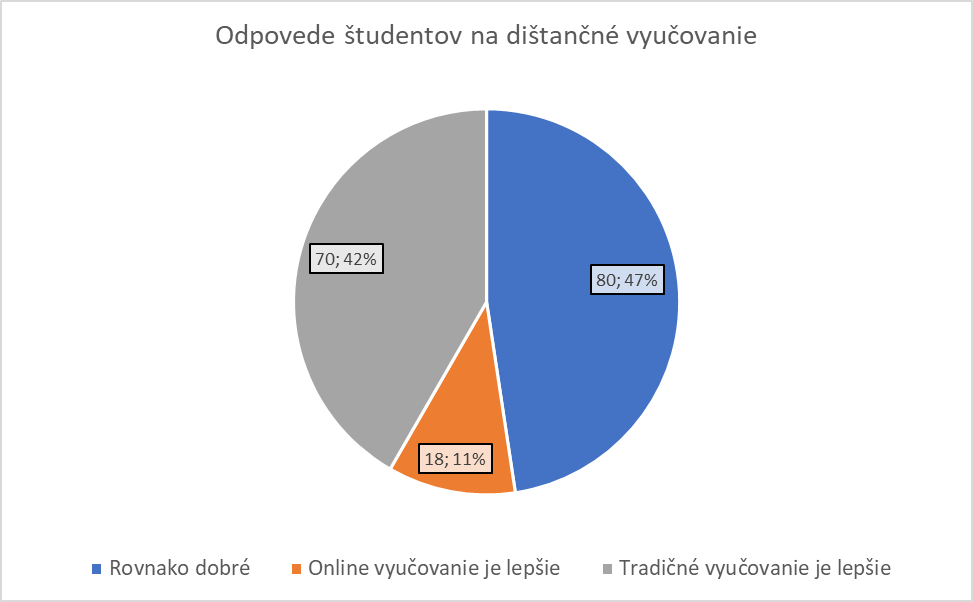
\includegraphics[scale=0.6]{d1.png}
%	\caption{Odpovede študentov na efektivitu vyučovania.}
%	\label{f:efektivitaStudenti}
%\end{figure*}

\section{Dopad dištančného vzdelávanie na tradičný spôsob} \label{dopad}
Už teraz je jasné, že aj keď dištančné vzdelávanie nemusí byť tak efektívne ako by sme očakávali alebo chceli, rozhodne ovplyvní tradičné vzdelávanie. Najpravdepobnejší prípad bude, že sa bude uskutočňovať kombinácia oboch spôsobov, a teda pôjde o kombinovanú výučba (alebo aj \textit{hybridnú výučba}) - niektoré školy už prestúpili na tento spôsob kvôli pandémii Covid-19\cite{Zimmerman:Experiment}.

%\subsection{Nejaké vysvetlenie} \label{ina:nejake}

%Niekedy treba uviesť zoznam:

%\begin{itemize}
%\item jedna vec
%\item druhá vec
%	\begin{itemize}
%	\item x
%	\item y
%	\end{itemize}
%\end{itemize}

%Ten istý zoznam, len číslovaný:

%\begin{enumerate}
%\item jedna vec
%\item druhá vec
%	\begin{enumerate}
%	\item x
%	\item y
%	\end{enumerate}
%\end{enumerate}

%\paragraph{Veľmi dôležitá poznámka.}
%Niekedy je potrebné nadpisom označiť odsek. Text pokračuje hneď za nadpisom.

\section{Záver} \label{zaver} % prípadne iný variant názvu



%\acknowledgement{Ak niekomu chcete poďakovať\ldots}


% týmto sa generuje zoznam literatúry z obsahu súboru literatura.bib podľa toho, na čo sa v článku odkazujete
\bibliography{literatura}
\bibliographystyle{plain} % prípadne alpha, abbrv alebo hociktorý iný
\end{document}
